\documentclass[12pt]{article}
\pagenumbering{gobble}
\linespread{1.15}

\usepackage{amsfonts}
\usepackage{amsmath}
\usepackage{amssymb}
\usepackage{array}
\usepackage{fancyhdr}
\usepackage{textcomp}
\usepackage{pgfplots, pgfplotstable}
\usepackage[margin=1in,headheight=10mm]{geometry}

\usetikzlibrary{datavisualization.formats.functions}

\pgfplotsset{compat=newest}

\pgfplotsset{
    SlopeField/.style={
        axis x line = middle,
        axis y line = middle,
        axis equal image, % Unit vectors for both axes have the same length
        view={0}{90}, % We need to use "3D" plots, but we set the view so we look at them from straight up
        samples=11, % How many arrows?
        cycle list={    % Plot styles
                blue,
                quiver={
                    u={1/\length}, v={f(x,y)/\length}, % End points of the arrows
                        scale arrows=0.3,
                        every arrow/.append style={
                           -latex % Arrow tip, uncomment to get "arrows" instead of line segments
                    },
                }\\
            }
    }
}

\newcommand{\contradiction}{%
    \ensuremath{{\Rightarrow\mspace{-2mu}\Leftarrow}}%
}

\newcommand{\angleb}[1]{\left\langle#1\right\rangle}
\newcommand{\vertb}[1]{\left\vert#1\right\vert}

\def\test#1{%
\expandafter\ifnum#1<0 -1 \else 1 \fi
}

\begin{document}
\pagestyle{fancy}
\fancyhead{}
\fancyhead[L]{Alexander Agruso}
\fancyhead[R]{MATH 3323 Homework 1}

\normalsize
\section*{Chapter 1.1}
\begin{itemize}
    \item [4.)] The slope field for $y'=1+2y$:

    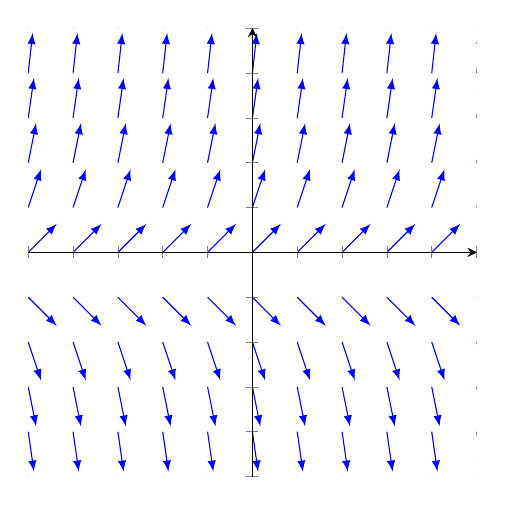
\begin{tikzpicture}[declare function={f(\x,\y)=1+2*\y;}]
        \def\length{sqrt(1+(f(x,y))^2)*3}
        \begin{axis}[
            SlopeField,
            xmin=-5, xmax=5,
            ymin=-5, ymax=5,
            zmin=0, zmax=1,
            domain=-5:5, y domain=-5:5,
            xtick={-5,-4,...,5}, ytick={-5,-4,...,5}
        ]
            \addplot3 (x,y,0);
        \end{axis}
    \end{tikzpicture}

    If $y=-\frac{1}{2}$, then as $t\rightarrow\infty$, $y$ will remain $-\frac{1}{2}$. If $y>-\frac{1}{2}$, then $y$ will approach $\infty$, and if $y<-\frac{1}{2}$, $y$ will approach $-\infty$.

    \item [11.)] j

    \item [12.)] c

    \item [13.)] g

    \item [14.)] b

    \item [15.)] h

    \item [16.)] e
\end{itemize}

\section*{Chapter 1.3}
\begin{itemize}
    \item [1.)] $2^{\text{nd}}$ order, linear

    \item [2.)] $2^{\text{nd}}$ order, nonlinear

    \item [3.)] $4^{\text{th}}$ order, linear

    \item [4.)] $2^{\text{nd}}$ order, nonlinear

    \item [5.)] $\dfrac{d^2}{dt^2}\left[e^t\right]=e^t$, $e^t-e^t=0$,\newline
    $\dfrac{d^2}{dt^2}\left[\cosh t\right]=\cosh t$, $\cosh t-\cosh t=0$,\newline
    Thus $e^t$ and $\cosh t$ are valid solutions.

    \item [6.)] $\dfrac{d}{dt}\left[e^{-3t}\right]=-3e^{-3t}$, $\dfrac{d^2}{dt^2}\left[e^{-3t}\right]=9e^{-3t}$, $9e^{-3t}-6e^{-3t}-3e^{-3t}=9e^{-3t}-9e^{-3t}=0$,\newline
    $e^t+2e^t-3e^t=3e^t-3e^t=0$,\newline
    Thus $e^{-3t}$ and $e^t$ are valid solutions.

    \item [11.)] Since $\dfrac{d}{dt}\left[e^{rt}\right]=re^{rt}$, we can substitute and find that $re^{rt}+2e^{rt}=0$, thus $r+2=0$, thus $r=-2$.
\end{itemize}

\end{document}
